%----------------------------------------------------------------------------------
% Exemplo do uso da classe tcc.cls. Veja o arquivo .cls
% para mais detalhes e instruções.
%----------------------------------------------------------------------------------

% PARA PREENCHIMENTO DO REVISOR:
% CHECKLIST
% [ ] Introduction: check the introduction 
    % [ ] Avoid jargon: Do you avoid jargon that is only explain in the rest of the text?
    % [ ] Clarity: Can anyone from computer science read the introduction and understand what's the objective?
    % [ ] Does it clearly describe the problem?
    % [ ] Does the introduction clearly state the contributions?

\sigla{COLREGS}{Collision Regulations at Sea}
\sigla{LSA}{Laboratório de Sistemas Autônomos}
\sigla{USV}{Unmanned Surface Vehicle}
\sigla{VO}{Velocity Obstacles}

\chapter{Introdução}\label{chap1:intro}
    A tecnologia está em constante evolução. Nos últimos anos, avanços significativos em robótica e em inteligência artificial contribuíram para que pesquisas no desenvolvimento de veículos de superfície aquática não tripulados (do inglês \textit{"Unmanned Surface Vehicle"} - USV) ganhassem atenção~\cite{HUANG2020451}. Um USV é definido por atuar de forma autônoma através de um sistema embarcado ou controlado remotamente~\cite{SONG2018351}. Conduzidas por frentes militares, científicas e privadas, pesquisas no desenvolvimento de USVs têm o intuito de auxiliar em atividades como monitoramento, comércio, exploração e pesquisas~\cite{JURAK2020}. Com o emprego de USVs tais atividades poderiam possuir maior duração e acurácia, além do custo de manutenção ser reduzido~\cite{LIU201671}. Porém, aspirar essa série de atividades para um USV fará com que sua atuação ocorra em cenários compartilhados com outras embarcações~\cite{KUWATA2014110}.

    Sob responsabilidade da Organização Internacional da Marinha (do inglês \textit{"Internation Marine Organization"} - IMO), as regulamentações de prevenção de colisões no mar (do inglês \textit{"COLlision REGulations at Sea"} - COLREGS) definem como as embarcações devem agir em situações de colisão~\cite{JURAK2020}. Visto que investigações apontam que acidentes marítimos acontecem principalmente pela violação das COLREGS~\cite{SONG2018351}, é importante considerar a implementação das mesmas no desenvolvimento de USVs. Dada a frequência de colisões e a gravidade das consequências, acidentes entre embarcações se torna uma preocupação latente~\cite{HUANG2019142}, e evadir de tais situações é um desafio no desenvolvimento de USVs~\cite{JURAK2020}. 

    Apesar da necessidade de considerar COLREGS no desenvolvimento de USVs, elas foram pensadas para serem compreendidas por humanos, que podem condicionar a sua aplicação à cada caso~\cite{KUWATA2014110}. Na Figura~\ref{fig:Kuwata2014_colregsInterpretation}, conforme apresentada por Kuwata \etal~\cite{KUWATA2014110}, é possível observar uma situação onde há risco de colisão (Figura~\ref{fig:Kuwata2014_colregApplicable}) e, portanto, deve-se aplicar as COLREGS. Uma situação semelhante porém sem risco de colisão é apresentada na Figura~\ref{fig:Kuwata2014_colregNA}, onde as COLREGS não são aplicáveis dado a velocidade das embarcações. Para identificar situações em que as COLREGS devem, ou não, ser aplicadas é preciso identificar que há um risco de colisão. Para isso, se utiliza um Índice de Risco de Colisão (do inglês \textit{"Collision Risk Index"} - CRI)~\cite{HUANG2019142}. Esse índice pode ser obtido através do método Ponto de Maior Aproximação (do inglês \textit{"Closest Point of Approach"} - CPA), que utiliza indicadores para determinar quando um encontro resultará em colisão. Após o êxito na detecção de uma situação de risco, é possível utilizar o algoritmo de Obstáculo de Velocidades (do inglês \textit{"Velocity Obstacles"} - VO). O que torna essa solução atraente é a possibilidade de resolver um encontro com diversas embarcações ao mesmo tempo e demanda pouco esforço computacional.
    
    Com base nas informações apresentadas e motivado pelo anseio de experienciar o processo científico, este trabalho visa explorar o CPA em conjunto com o VO utilizando uma metodologia de pesquisa baseada essencialmente em 
    \begin{enumerate*}[label=\alph*)]
        \item identificação do problema,
        \item entendimento do problema,
        \item proposta de solução,
        \item implementação da solução,
        \item validação da solução, e
        \item comparação dos resultados com outros autores.
    \end{enumerate*}
    Como resultado, é esperado uma aplicação capaz de identificar o risco de colisão entre embarcações em um determinado encontro utilizando CPA. Além disso, será realizada a integração em um sistema para USV já existente desenvolvido por Jurak~\cite{JURAK2020}, para que seja possível realizar simulações e analisar se o comportamento resultante está de acordo com o esperado. Nesse sistema também será acrescido a criação do VO como um obstáculo virtual sob a hipótese de aumentar a segurança do sistema.
    
    \begin{figure}
    \centering
    
        \begin{subfigure}{0.4\textwidth}
            \centering
            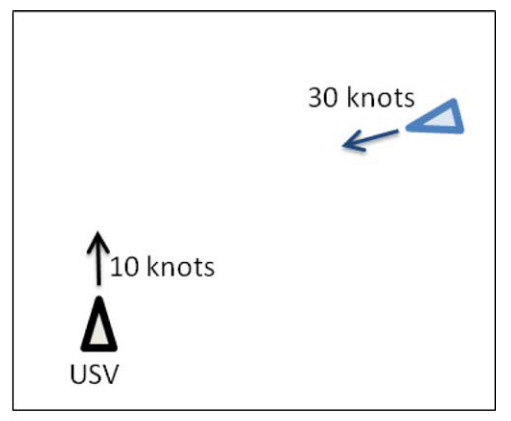
\includegraphics[width=\textwidth]{fig/chap1/colregs_applicable.png}
            \caption{}
            \label{fig:Kuwata2014_colregApplicable}
        \end{subfigure}
        \begin{subfigure}{0.4\textwidth}
            \centering
            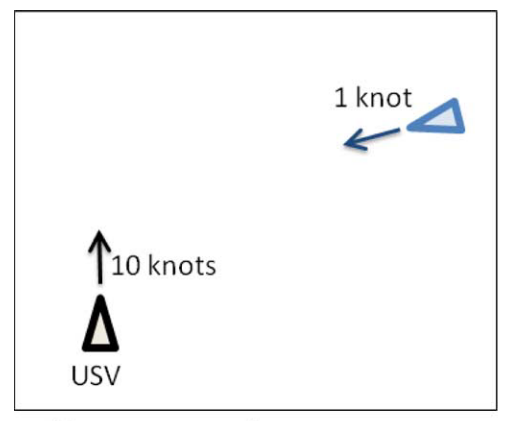
\includegraphics[width=\textwidth]{fig/chap1/colregs_na.png}
            \caption{}
            \label{fig:Kuwata2014_colregNA}
        \end{subfigure}
    
    \caption{Mesmo encontro para diferentes velocidades da embarcação que se aproxima (triângulo azul). Na figura (a) a COLREGS é aplicável e o USV (triangulo cinza) deve desviar da embarcação que se aproxima, enquanto que na figura (b) não é aplicável e o USV pode seguir sua rota sem alteração}
    \label{fig:Kuwata2014_colregsInterpretation}
    \end{figure}
    
    Como contribuição, este trabalho visa capacitar o sistema desenvolvido por Jurak~\cite{JURAK2020} a identificar situações de colisão através do CPA, tornando possível aplicar COLREGS apenas para encontros em que haverá colisão. Quando em situação de colisão, assim como no sistema de Jurak~\cite{JURAK2020}, sera criado um obstáculo virtual a partir do VO gerado pelo encontro. Essas implementações visam colabor para o aprimoramento dos barcos-robôs pertencentes ao Laboratório de Sistemas Autônomos (LSA) da PUCRS. Ademais, a maioria dos sistemas desenvolvidos para USVs ou são resguardados por patentes, ou então possuem acesso restrito àqueles que não participaram de seu desenvolvimento~\cite{JURAK2020}. Sendo assim, este trabalho visa contribuir à comunidade de desenvolvedores mantendo o que for desenvolvido em código aberto. 
    
    O presente documento está estruturado da seguinte forma: no capítulo \ref{chap1:intro}, além das informações já apresentadas, o trabalho proposto será aprofundado na sessão \ref{subchap1:trab_prop}, e as contribuições serão evidenciadas na sessão \ref{subchap1:contrib}. O capítulo \ref{chap2:fund_teo} contém uma revisão teórica apresentando maiores detalhes a respeito de USV na sessão \ref{subchap2:USV}, COLREGS na sessão \ref{subchap2:colregs} e prevenção de colisão na sessão \ref{subchap2:prev_col}.
    
